\subsection{Semesterticket}
Euer Studentenausweis berechtigt euch zur Fahrt auf vielen Zugstrecken in
Niedersachsen. Aktuelle Informationen zum Semesterticket gibt es auf den Seiten
des AStA (\nurl{http://www.asta.tu-bs.de/semesterticket.php}).
Unten seht ihr den Gültigkeitsbereich des Semestertickets im Großraum Hannover. 
Nach Norden und und Westen deckt das Semesterticket weitere Strecken ab. 
Einen grober Überblick gibt die nebenstehende Karte. 

Es d"urfen nur Regionalexpress (RE) und Regionalbahn (RB) der
Deutschen Bahn AG, sowie teilweise der Metronom in der zweiten Klasse
benutzt werden. Also NICHT Strecken der Nordwestbahn (NWB). Einen
genauen Überblick findet ihr in Form einer Streckenliste auf der
Seite \pageref{streckenliste1}.
%und \pageref{streckenliste2}. 

Mehr Details könnt ihr den Seiten des AStA
unter \url{http://www.asta.tu-bs.de/semesterticket.php} entnehmen.

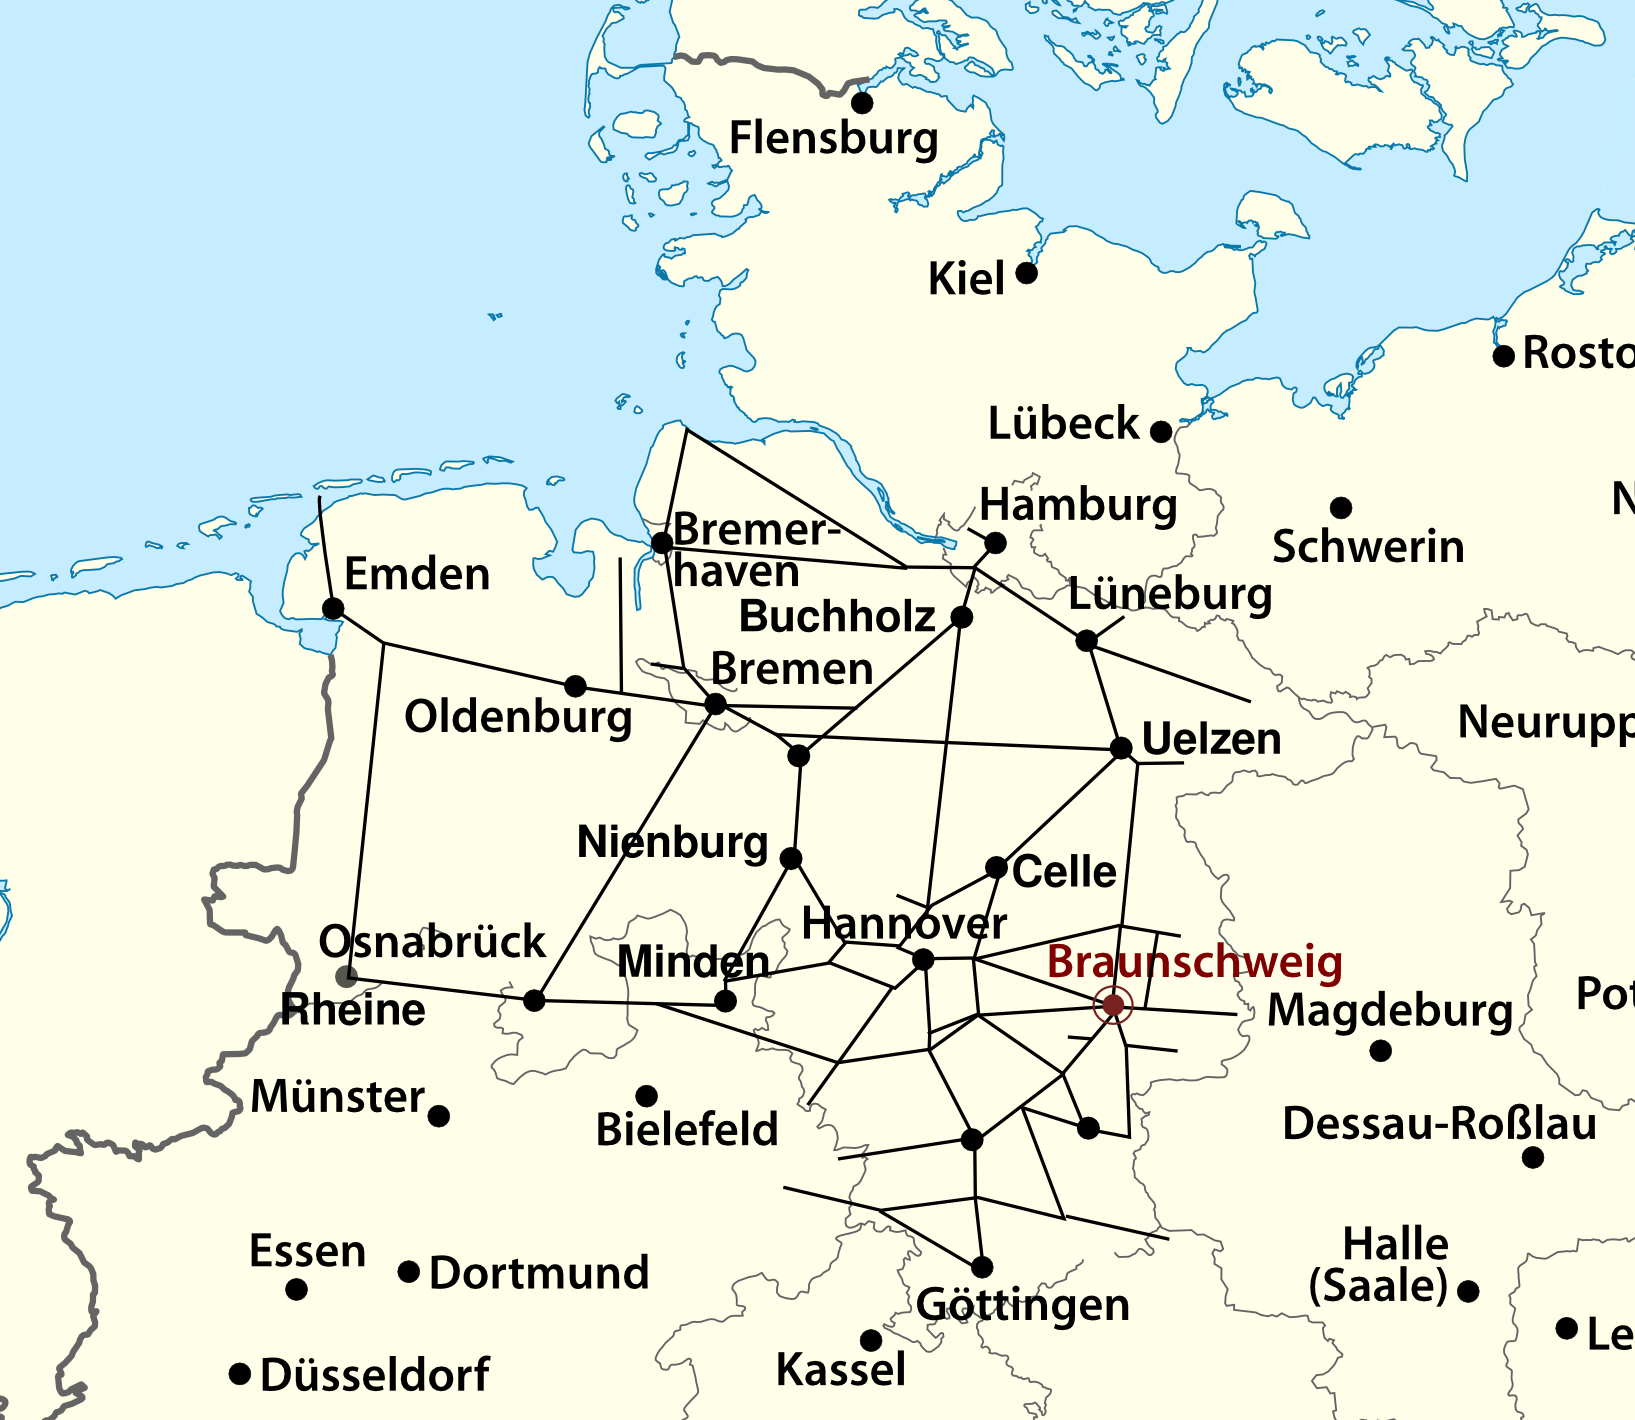
\includegraphics[width=\columnwidth]{bilder/ticket_deutschland.png}

\end{multicols}
%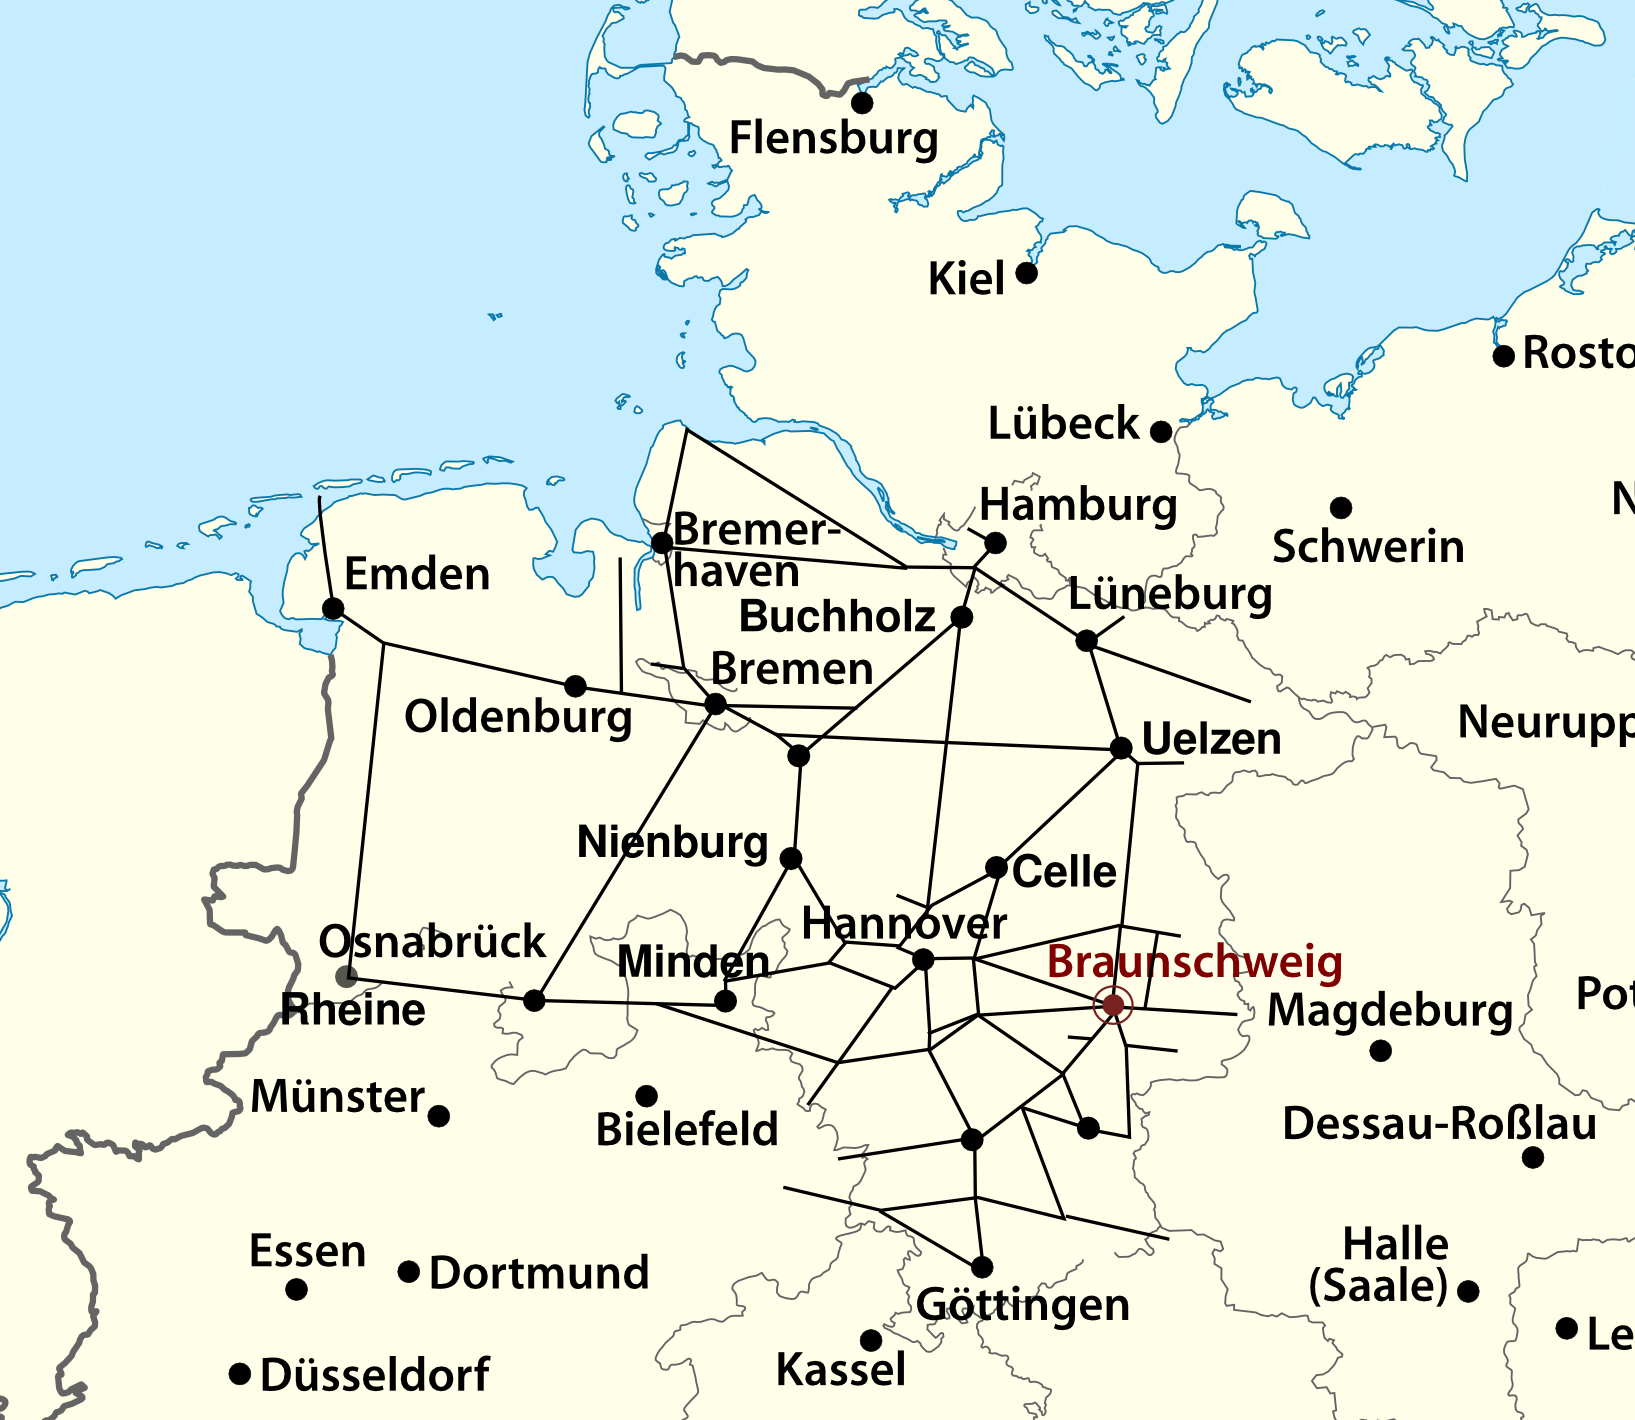
\includegraphics[scale=0.5]{bilder/ticket_deutschland}
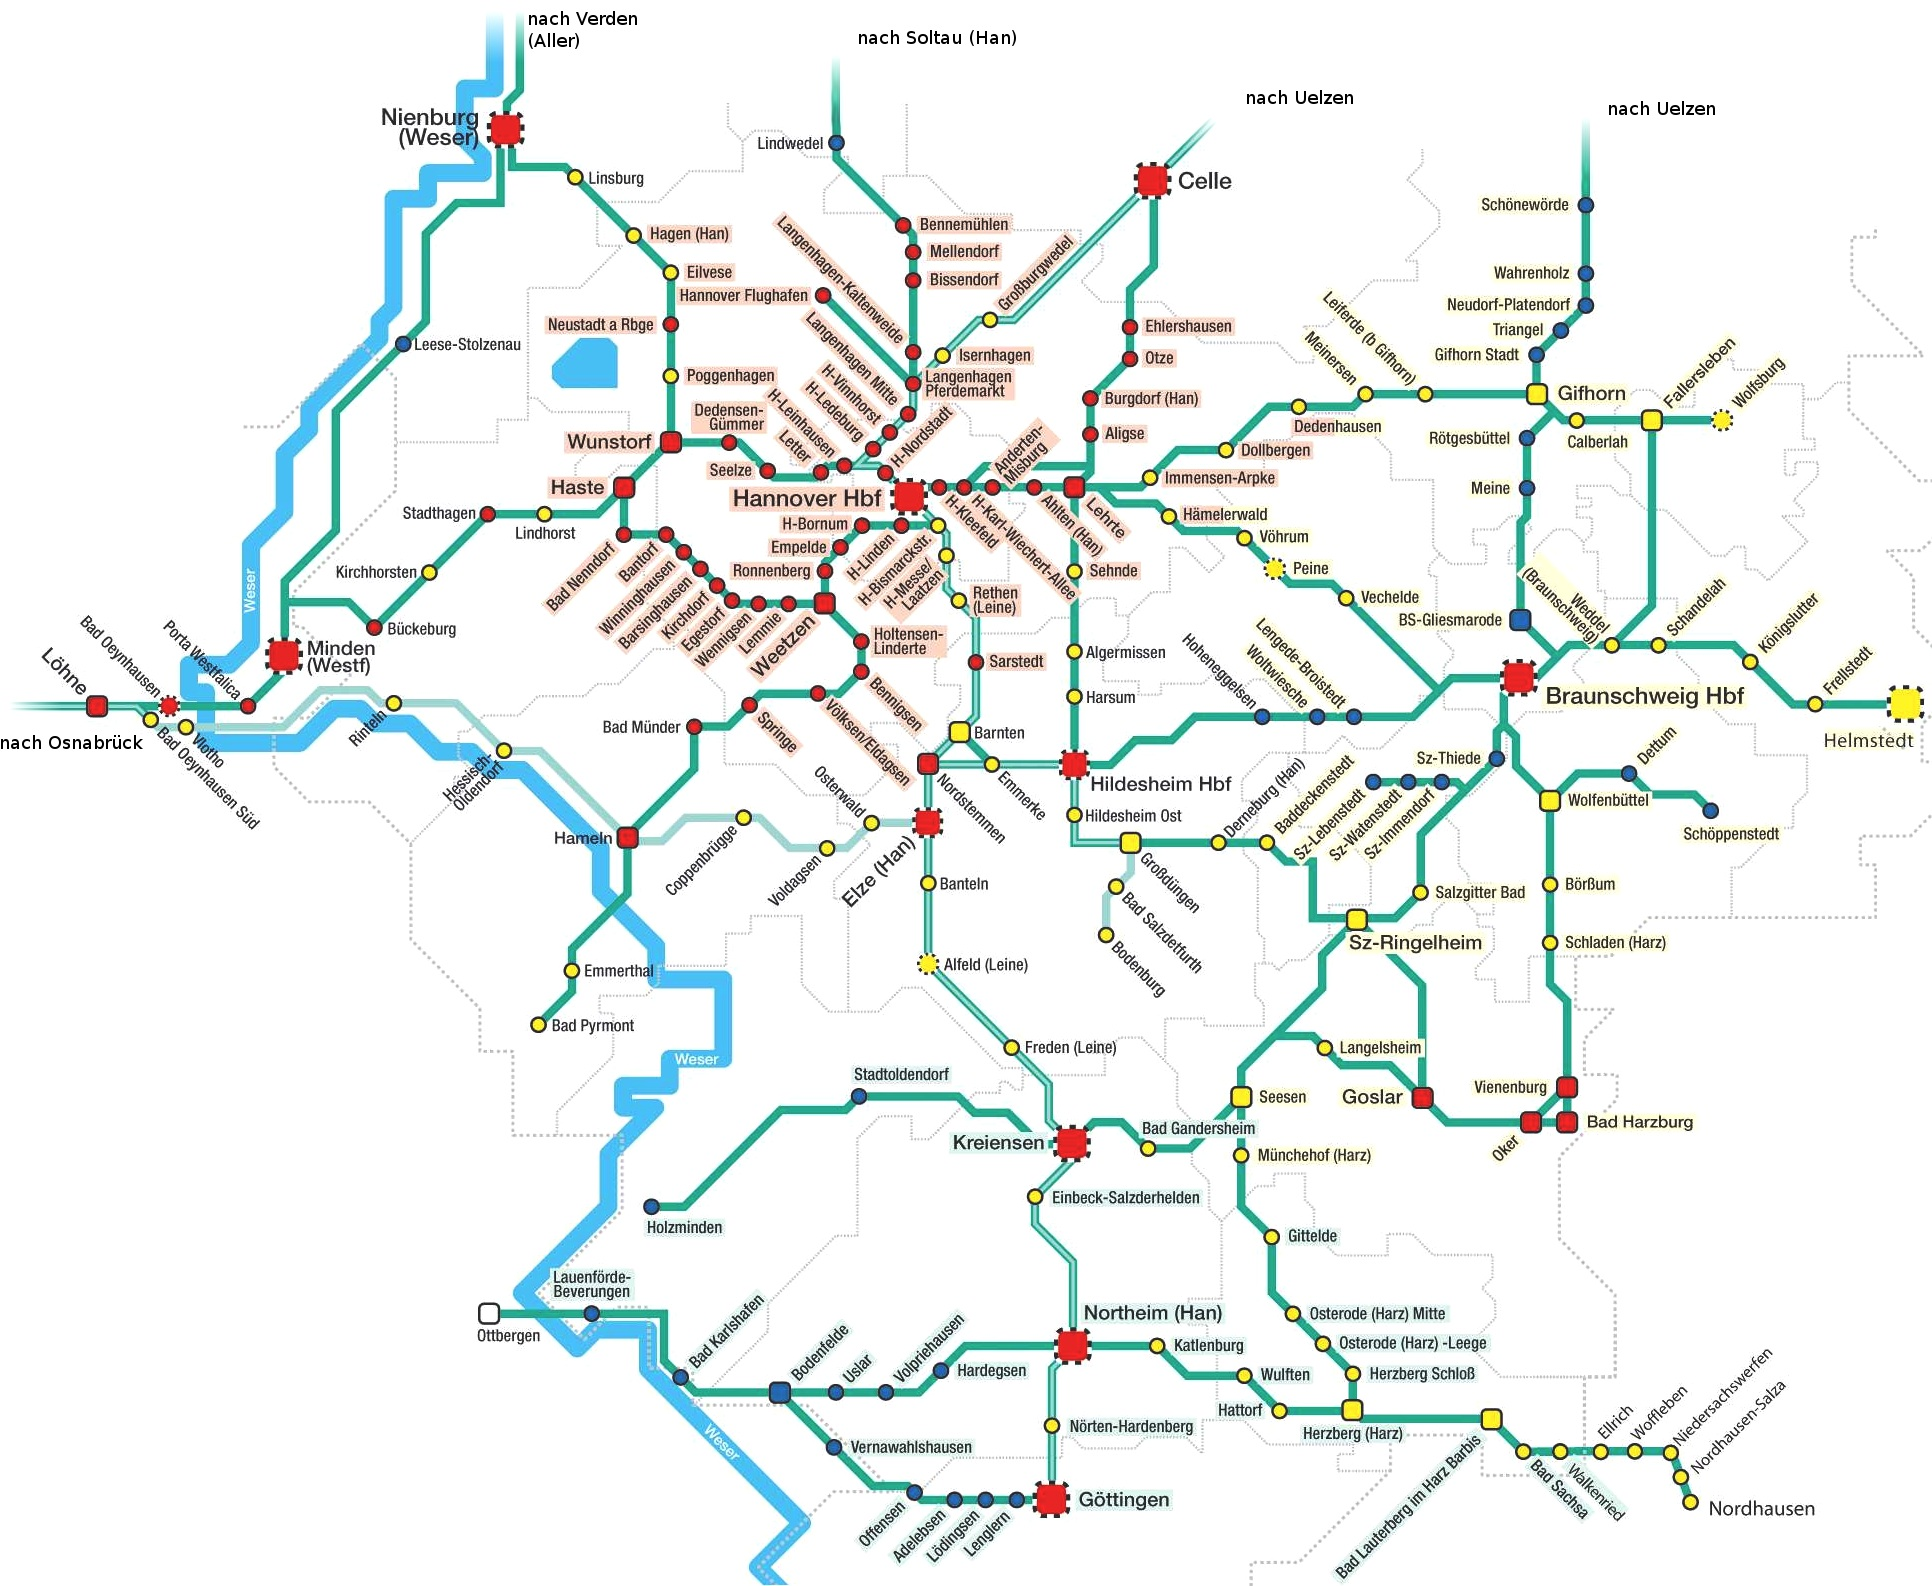
\includegraphics[width=\textwidth]{bilder/ticket_bis_11_Dezember.jpg}
\newpage
\newpage
\begin{multicols}{2}
\subsubsection*{Streckenübersicht Wintersemester 2010/2011 und Sommersemester 2011 gültig ab 1.10.2010}
\label{streckenliste1}
\begin{tabular}{|l|l|l|p{2cm}|}
\hline
\multicolumn{3}{|l|}{\textbf{Strecke/ Streckenabschnitt}}& \textbf{KbN}\\
\textbf{\textit{von}} & \textit{über} & \textbf{\textit{bis}} & \\ \cline{ 1- 4}
Lüneburg &  & Dannenberg Ost & 112 \\ \hline
Braunschweig Hbf & Gifhorn & Uelzen & 115 \\ \hline
Bremen Hbf & Soltau & Uelzen & 116 \\ \hline
Hamburg-Harburg &  & Stade & 121 \\ \hline
Buchholz (Nordheide) & Soltau & Bennemühlen & 123 \\ \hline
Minden Westf. & Nienburg & Rotenburg/Bremen Hbf & 124 \\ \hline
Bremen Hbf &  & Cuxhaven & 125 \footnotemark[1] \\ \hline
Bremen Hbf &  & Bremen-Vegesack & 126 \footnotemark[1] \\ \hline
Echem &  & Lüneburg & 145 \\ \hline
Hannover Hbf & Gifhorn & Wolfsburg Hbf & 300 \\ \hline
Braunschweig Hbf &  & Wolfsburg Hbf & 301 \\ \hline
Uelzen &  & Schnega & 305 \\ \hline
Hannover Hbf & Braunschweig Hbf & Helmstedt & 310 \\ \hline
Braunschweig Hbf & Wolfenbüttel & Schöppenstedt & 312 \footnotemark[2] \\ \hline
Braunschweig Hbf &  & Hildesheim Hbf & 313 \\ \hline
Hannover Hbf & Hildesheim Hbf/Goslar & Bad Harzburg & 320 \\ \hline
Braunschweig Hbf &  & Sz-Lebenstedt & 352 \\ \hline
Braunschweig Hbf & Wolfenbüttel/Vienenburg & Goslar & 353 \\ \hline
Holzminden & Kreiensen & Bad Harzburg & 354 \\ \hline
Ottbergen & Bodenfelde & Göttingen & 356.1 \\ \hline
Ottbergen & Bodenfelde & Northeim & 356.2 \\ \hline
Göttingen & Northeim & Walkenried & 357 \footnotemark[1] \\ \hline
Braunschweig Hbf & Seesen & Herzberg (Harz) & 358 \\ \hline
Haste & Hannover Hbf/Haste & Minden (Westf) & 360.1 \\ \hline
Nienburg (Weser) & Hannover Hbf & Haste & 360.2 \\ \hline
Hannover Hbf & Lehrte & Hildesheim Hbf & 360.3 \\ \hline
Bennemühlen & Hann./Sarstedt & Hildesheim Hbf & 360.4 \\ \hline
Bad Pyrmont & Hameln/Weetzen & Hannover-Flughafen & 360.5 \\ \hline
Celle & Lehrte & Hannover Hbf & 360.6.7 \\ \hline
Hannover Hbf &  & Hannover Bismarckstr. & 361 \footnotemark[1] \\ \hline
Hannover Hbf &  & Löhne (Westf.) & 370 \\ \hline
Löhne (Westf.) & Hameln & Hildesheim Hbf & 372 \\ \hline
Hildesheim Hbf &  & Bodenburg & 373 \\ \hline
Salzbergen & Osnabrück Hbf & Minden (Westf.) & 375 \footnotemark[1] \\ \hline
Bremen Hbf &  & Hannover Hbf & 380 \\ \hline
Osnabrück Hbf &  & Bremen Hbf & 385 \footnotemark[1] \\ \hline
Norddeich Mole & Oldenburg (Oldb) & Bremen Hbf & 390 \footnotemark[1] \\ \hline
Norddeich Mole & Meppen & Rheine & 395 \footnotemark[1] \\ \hline
Emden Hbf &  & Emden Außenhafen & 396 \\ \hline
Leer (Ostfr.) &  & Weener & 397 \\ \hline
\end{tabular}

\footnotetext[1]{nur in den Zügen der DB Regio AG, also nicht in Zügen der Nordwestbahn}
\footnotetext[2]{gültig auch in Bus von  Schöppenstedt-Schöningen-Helmstedt}
\end{multicols}
\begin{multicols}{2}
